% Template article for preprint document class `elsart'
% SP 2001/01/05

%\documentclass{elsart}

% Use the option doublespacing or reviewcopy to obtain double line spacing
\documentclass[doublespacing]{elsart}
\setlength{\textwidth}{6.5true in}
% check for the existence of the variable pdfoutput
\newif\ifpdf
 \ifx\pdfoutput\undefined
   \pdffalse % we are not running PDFLaTeX
 \else
   \pdfoutput=1 % we are running PDFLaTeX
   \pdftrue
 \fi

% if you use PostScript figures in your article
% use the graphics package for simple commands
% \usepackage{graphics}
% or use the graphicx package for more complicated commands

 %Then use your new variable \ifpdf
 \ifpdf
   \usepackage[pdftex]{graphicx}
   \pdfcompresslevel=9
   \DeclareGraphicsExtensions{.pdf,.mps,.png,.jpg}
 \else
    \usepackage[dvips]{graphicx}
    \DeclareGraphicsExtensions{.eps,.ps,.bmp,.tif,.tiff,.tga}
 \fi

\graphicspath{{./figures/}}

% or use the epsfig package if you prefer to use the old commands
% \usepackage{epsfig}

% The amssymb package provides various useful mathematical symbols
\usepackage{amssymb}

% The rotating package allows one to rotate tables and figures
\usepackage{rotating}

% The rcsinfo package allows one to access rcs strings
%\usepackage[fancyhdr]{rcsinfo}
\usepackage{rcsinfo}

% The lgrind package allows formatting of program listings
%\usepackage{lgrind}

\bibliographystyle{elsart-num}

% User-defined macros

\newcommand{\udfcount}{\ensuremath{N^{udf}_{i}}}
\newcommand{\udftime}{\ensuremath{\tau^{udf}_{i}}}
\newcommand{\verlettime}{\ensuremath{\tau_{verlet}}}
\newcommand{\sitecount}{\ensuremath{{N_{sites}}}}
\newcommand{\rcutoff}{\ensuremath{r_{c}}}
\newcommand{\density}{\ensuremath{\rho}}
\newcommand{\nonbondtime}{\ensuremath{\tau_{non-bond}}}
\newcommand{\nodecount}{\ensuremath{p}}
\newcommand{\allreducetime}{\ensuremath{\tau_{AllReduce}(\sitecount,\nodecount)}}
\newcommand{\globalizepostime}{\ensuremath{\tau_{Globalize}(\sitecount, \nodecount)}}
\newcommand{\meshsize}[1]{\ensuremath{N_{#1}}}
\newcommand{\nodemeshsize}[1]{\ensuremath{\nodecount_{#1}}}
\newcommand{\meshpernode}[1]{\ensuremath{n_{#1}}}
\newcommand{\nodecoord}[1]{\ensuremath{c_{#1}}}
\newcommand{\pmetime}{\ensuremath{\tau_{p3me}(\nodecount,\meshsize{mesh})}}

% End of user defined macros

% settings to cause rcsinfo information to be shown in footer
%% remove this prior to final printing
%\pagestyle{fancyplain}
%\fancyhead[R]{\leftmark}
%\fancyhead[LE,RO]{\thepage}

%% end of section that should be removed prior to final printing

\begin{document}

\rcsInfo $Id: jpdc_bg.tex 5037 2003-04-15 03:56:05Z germain $


\begin{frontmatter}

% Title, authors and addresses

% use the thanksref command within \title, \author or \address for footnotes;
% use the corauthref command within \author for corresponding author footnotes;
% use the ead command for the email address,
% and the form \ead[url] for the home page:
%\title{Blue Matter, An Application Framework for Molecular Simulation on Blue Gene\thanksref{http://www.research.ibm.com/bluegene}}
\title{Blue Matter, An Application Framework for Molecular Simulation on Blue Gene\thanksref{acks}}
% \thanks[label1]{}
\thanks[acks]{The authors wish to acknowledge many useful discussions
with Bruce J. Berne and Glenn J. Martyna regarding molecular dynamics
algorithms and members of the BG/L hardware and systems software
teams, particularly Alan Gara, Philip Heidelberger, Burkhard
Steinmacher-Burow, and Mark Giampapa, as well as the contributions of
Huafeng Xu at the early stages of this project. We also wish to thank
the anonymous referees for their feedback on this paper.}
\thanks[yuk_in_mn]{Current address:\\ University of Minnesota\\
Supercomputing Institute for Digital Simulation and Advanced
Computation\\ 599 Walter Library\\ 117 Pleasant Street S.E.\\
Minneapolis, MN 55455}

%\author{Name\corauthref{cor1}\thanksref{label2}}
\author[ykt]{B.G. Fitch}
\author[ykt]{R.S. Germain}
\author[toronto]{M. Mendell}
\author[arc]{J. Pitera}
\author[ykt]{M. Pitman}
\author[ykt]{A. Rayshubskiy}
\author[ykt]{Y. Sham\thanksref{yuk_in_mn}}
\author[ykt]{F. Suits}
\author[arc]{W. Swope}
\author[ykt]{T.J.C. Ward}
\author[ykt]{Y. Zhestkov}
\author[ykt]{R. Zhou}
% \ead{email address}
%\ead[url]{http://www.research.ibm.com/bluegene}
% \thanks[label2]{}
% \corauth[cor1]{}
% \address{Address\thanksref{label3}}
\address[ykt]{IBM Thomas J. Watson Research Center\\
P.O. Box 218\\
Yorktown Heights, NY 10598}
% \thanks[label3]{}


% use optional labels to link authors explicitly to addresses:
% \author[label1,label2]{}
% \address[label1]{}
% \address[label2]{}

%\author{}

%\address{}

\address[arc]{IBM Almaden Research Center\\
650 Harry Road\\
San Jose, CA 95120-6099}

\address[toronto]{IBM Canada\\
8200 Warden Avenue\\
Markham, ON L6G 1C7}

%\address[umn]{University of Minnesota\\
%Supercomputing Institute for Digital Simulation and Advanced Computation\\
%599 Walter Library\\
%117 Pleasant Street S.E.\\
%Minneapolis, MN 55455}

\title{}

\begin{abstract}
% Text of abstract
In this paper we describe the context, architecture, and challenges of
Blue Matter, the application framework being developed in conjunction
with the science effort within IBM's Blue Gene project.  The study of
the mechanisms behind protein folding and related topics can require
long time simulations on systems with a wide range of sizes and the
application supporting these studies must map efficiently onto a large
range of parallel partition sizes to optimize scientific throughput
for a particular study. The design goals for the Blue Matter
architecture include separating the complexities of the parallel
implementation on a particular machine from those of the scientific
simulation as well as minimizing system environmental dependencies so
that running an application within a low overhead kernel with
minimal services is possible.  We describe some of the parallel
decompositions currently being explored that target the first member
of the Blue Gene family, BG/L, and present simple performance models
for these decompositions that we are using to prioritize our
development work. Preliminary results indicate that the high
performance networks on BG/L will allow us to use FFT-based
techniques for periodic electrostatics with reasonable speedups on
512-1024 node count partitions even for systems with as few as 5000 atoms.
\end{abstract}

\begin{keyword}
% keywords here, in the form: keyword \sep keyword

% PACS codes here, in the form: \PACS code \sep code
  \PACS
\end{keyword}
\end{frontmatter}

% main text
%\section{}
%\label{}

% The Appendices part is started with the command \appendix;
% appendix sections are then done as normal sections
% \appendix

% \section{}
% \label{}

\setlength{\headheight}{28pts}

\section{Introduction}

In December 1999, IBM announced the start of a five year effort to
build a massively parallel computer to be applied to the study of
biomolecular phenomena such as protein folding.\cite{allen:2001} The
project has two goals: advancing our understanding of the mechanisms
behind biologically important phenomena such as protein folding via
large scale simulation and exploring novel ideas in massively parallel
machine architecture and software.  This project should enable
biomolecular simulations that are orders of magnitude larger and
longer than current technology permits. The first member of the Blue
Gene machine family is Blue Gene/L, for which a 512 node prototype is
projected to become available in the second half of 2003, with a fully
operational machine scheduled for the 2004-2005 time frame. The
machine architecture has evolved significantly since the inception of
the project, but one aspect that has remained constant is the use of a
three dimensional mesh interconnect topology, a feature that may
require the application to be aware of the machine topology in order
to achieve optimal performance.  This has not been the case for other
recent large parallel machines such as ASCI White.  Another unusual
feature of this machine is the availability of a second high
performance interconnect network to provide low-latency and high
bandwidth global broadcast and reduction capabilities.  More details
about the machine that are most relevant to an application developer
are provided in the body of this paper and additional information can
be found in a recent paper by the Blue Gene team\cite{bgl_sc:2002}.
The study of the mechanisms behind protein folding and related topics
can require long time simulations on systems with a wide range of
sizes and the application supporting these studies must map
efficiently onto a large range of parallel partition sizes to optimize
scientific throughput for a particular study. Typical system sizes of
interest range from 5000 atoms (for a small peptide in water) through
30,000 atoms (for a folded 200-residue protein in water) up to 200,000
atoms or more (for a protein-membrane system or large unfolded protein
in water).

To support the goals of the Blue Gene project related to protein
science and to explore novel application programming approaches for
massively parallel machine architectures in the context of a concrete
problem, we have been working on an application framework, Blue
Matter, which is currently focused on biomolecular simulation. It is
hoped that the lessons learned and even some of the components
developed can be reused in other application domains.  One of the
principal design goals for this framework is the effective logical
separation of the complexities of programming a massively parallel
machine from the complexities of biomolecular simulation through the
definition of appropriate interfaces.  Encapsulation of the semantics
of the biomolecular simulation methodologies means that the
application can track the evolution of the machine architecture and
explorations of various parallel decomposition schemes can take place
with minimal intervention from the domain experts on the team, who are
also the end users of the Blue Matter application. Furthermore, we
have decomposed the application into a core parallel engine with
minimal system environmental requirements running on BG/L and a set of
support modules providing setup, monitoring, and analysis
functionality that can run on other host machines.  Minimizing system
environmental requirements for the core parallel engine enables the
use of non-pre-emptive low overhead parallel operating system (OS)
kernels\cite{fitch:1993} to enable scalability to thousands of nodes.

In order to prioritize our development efforts, we are exploring
various mappings of the Blue Matter application onto the BG/L platform
via simple models.  One area of interest is the exploitation of the
high performance networks available on Blue Gene/L in a way that
minimizes potential software overheads.  If we can find parallel
decompositions that directly take advantage of the hardware
communications facilities, we will reduce the software overheads that
may limit the maximum partition for a fixed size problem, thereby
maximizing throughput for a given molecular simulation.

\subsection{Machine Overview}

Blue Gene/L is a cellular architecture machine built of nodes
containing a single application-specific integrated circuit (ASIC) and
additional off-chip memory.  Each ASIC has two IBM PowerPC processors
with a projected clock speed of 700~MHz as well as cache memory and
communications logic.  The target configuration contains a maximum of
$65,536$ compute nodes with several communications networks.  The
networks that are of primary interest to application developers are
the three-dimensional torus that connects each node to its six nearest
neighbors with a link bandwidth of 175~MB/s bidirectional
(2~bits/cycle), a physically separate global combining/broadcast tree
with bandwidth of 350~MB/s (4~bits/cycle) and a 1.5 microsecond
one-way latency on a 64K node partition, and a global
barrier/interrupt network.  BG/L can be electronically partitioned
into multiple systems with a currently envisioned minimum size of 512
nodes, each of which has its own complete set of networks.  The target
peak performance of the full $65,536$ node configuration of BG/L is
180/360~TeraFLOPs, where the lower number corresponds to scenarios in
which one processor exclusively handles communication tasks, and the
larger number assumes the application can take full advantage of both
processors for computation.

\subsection{Blue Gene Science}

Understanding the physical basis of protein function is a central
objective of molecular biology.  Proteins function through internal
motion and interaction with their environment. An understanding of
protein motion at the atomic level has been pursued since the earliest
simulations of their dynamics \cite{karplus:2002}.  When simulations
can connect to experimental results, the microscopic view of processes
revealed by simulation acquire more credibility and the simulation
results can help interpret the experimental data \cite{nagle:2000}.
Improvements in computational power and simulation methods have led to
important progress in studies of protein structure, thermodynamics, and
kinetics\cite{karplus:2002,sheinerman:98,duan:1998,snow:2002}.

\subsection{Methodological Implications for the Application}

The validity of a molecular simulation depends strongly on the the
quality of the force field, including the representation of water, the
treatment of long-range intermolecular interactions, and the simulated
environment of the protein.  Validity comes at a cost, however, both
in the computational expense of the simulation and the complexity of
the molecular dynamics (MD) software.

Biological molecules are surrounded by water, so the representation of
water in a simulation has a critical effect on its quality.  Explicit
solvent simulations represent the atoms of each of the water molecules
around a protein, and calculate all of the intermolecular forces and
dynamics associated with those atoms.  The expense of explicit water
is significant since the number of atoms contributed by the solvent
can far exceed that of the protein itself.  In order to avoid boundary
effects in explicit water simulations, it is typical to treat the
simulated system with periodic boundary conditions.  Alternatively,
implicit solvent models of various levels of sophistication have been
used which typically represent the water as a continuum dielectric,
optionally coupled with a cavity surface tension term to model the
hydrophobic effect.  Although implicit solvent models have produced
important results in some areas, there are important cases where
significant differences exist in the results obtained from an implicit
as opposed to an explicit treatment of water\cite{zhou:2002}.
 
A major feature of molecular simulation that poses an implementation
challenge is the treatment of long-range interactions.  For biological
systems, this term arises from the long-ranged Coulombic interaction
between charged amino acids or ions.  A simplification is to only
include the interactions of atoms within a short cutoff radius of each
other, which reduces the computational burden, but in systems with
charged groups or free charges this approach can lead to unphysical
artifacts\cite{bader:1992}.  The periodic representations used for
explicit solvent simulations can be treated correctly with the use of
the Ewald summation technique\cite{leeuw:1980} or related
methods\cite{hockney:1988} which typically require the use of Fourier
transform techniques.  These techniques introduce global data
dependencies and are correspondingly complex to parallelize
efficiently.  Nonetheless, this addition to the MD code is important
for the accuracy of the results and these techniques, with their
scalability consequences, are essential for large scale simulations
that can match experiment.

Another feature in molecular simulation that demands added complexity
is the specific ensemble being simulated, e.g. whether the simulated
system is in a constant pressure or constant volume environment, and
whether or not it is coupled to a heat bath. Supporting these
capabilities requires additional code, communication, and added
barriers to synchronize the execution of parallel tasks.  In
particular, the calculation of the instantaneous internal "pressure"
inside the simulation cell requires a global reduction of all the
interparticle forces projected along their displacements from the
origin.

\section{Application Architecture}
\subsection{Overview}

Blue Matter is a software framework for performing biomolecular
simulations primarily targeting parallel computing platforms
containing thousands of nodes.  At the highest level, the Blue Matter
architecture specifies a modular decomposition and has been
implemented as independent subprograms that cooperate via architected
interfaces. By using concepts from generic
programming\cite{austern:1999} and defining appropriate interfaces, we
have been working towards a separation of the complexity of molecular
dynamics simulation from the complexity of parallel programming with
minimal impact on performance.  The Blue Matter architecture requires
infrastructure to support extensive regression and validation because
of the aggressive and experimental nature of the computational
platform we are targeting.  As part of the effort to separate the
molecular dynamics domain from the implementation of the framework, it
is essential that functional correctness be established by validating
the results of test simulations rather than by examining code.

Figure~\ref{fig:bluematter_overview} shows the relationship between
the major modules in the Blue Matter framework.  A representation of
the molecular system and its associated simulation parameters is
created in a relational database as part of the set up process.  This
representation forms part of the experimental record which, along with
information about specific simulation runs such as hardware platform
type and configuration, can be accessed during analyses of the
simulation data.  A kernel generation module retrieves the data
associated with a particular molecular system from the database and
creates a Molecular System Definition (MSD) file containing C++ code
which is then compiled and linked with framework source code libraries
to produce an executable.  While running on a suitable platform, the
executable sends data to a host computer for consumption by analysis
and monitoring modules via a raw datagram (RDG) stream.

The Blue Matter framework has been architected to allow exploration of
multiple application decompositions with each implementation reusing
the domain specific modules and semantics.  Currently, this framework
is specialized by selecting force field functional forms and
simulation methods.  Our strategy for separating MD complexity from
parallel complexity includes factoring as much domain specific
knowledge as possible into the setup phase.  The framework is designed
to manipulate domain function in very fine grained functional units,
embodied by call-back functions that we refer to as User Defined
Functions (UDFs), that encapsulate localized domain specific data
transformations.  The call-backs are resolved at compile-time rather
than run-time for performance reasons.  Flexibly managing the
granularity of the domain decomposition is important because of the
range of node count and molecular system sizes we are targeting.
Implementing a new parallel decomposition or communications pattern in
this framework does not involve changing the UDFs or restating the
simulation semantics.  Using this generic infrastructure, we are able
to support several force fields and map them onto drivers suitable to
the computational platform available.

\begin{sidewaysfigure}[p]
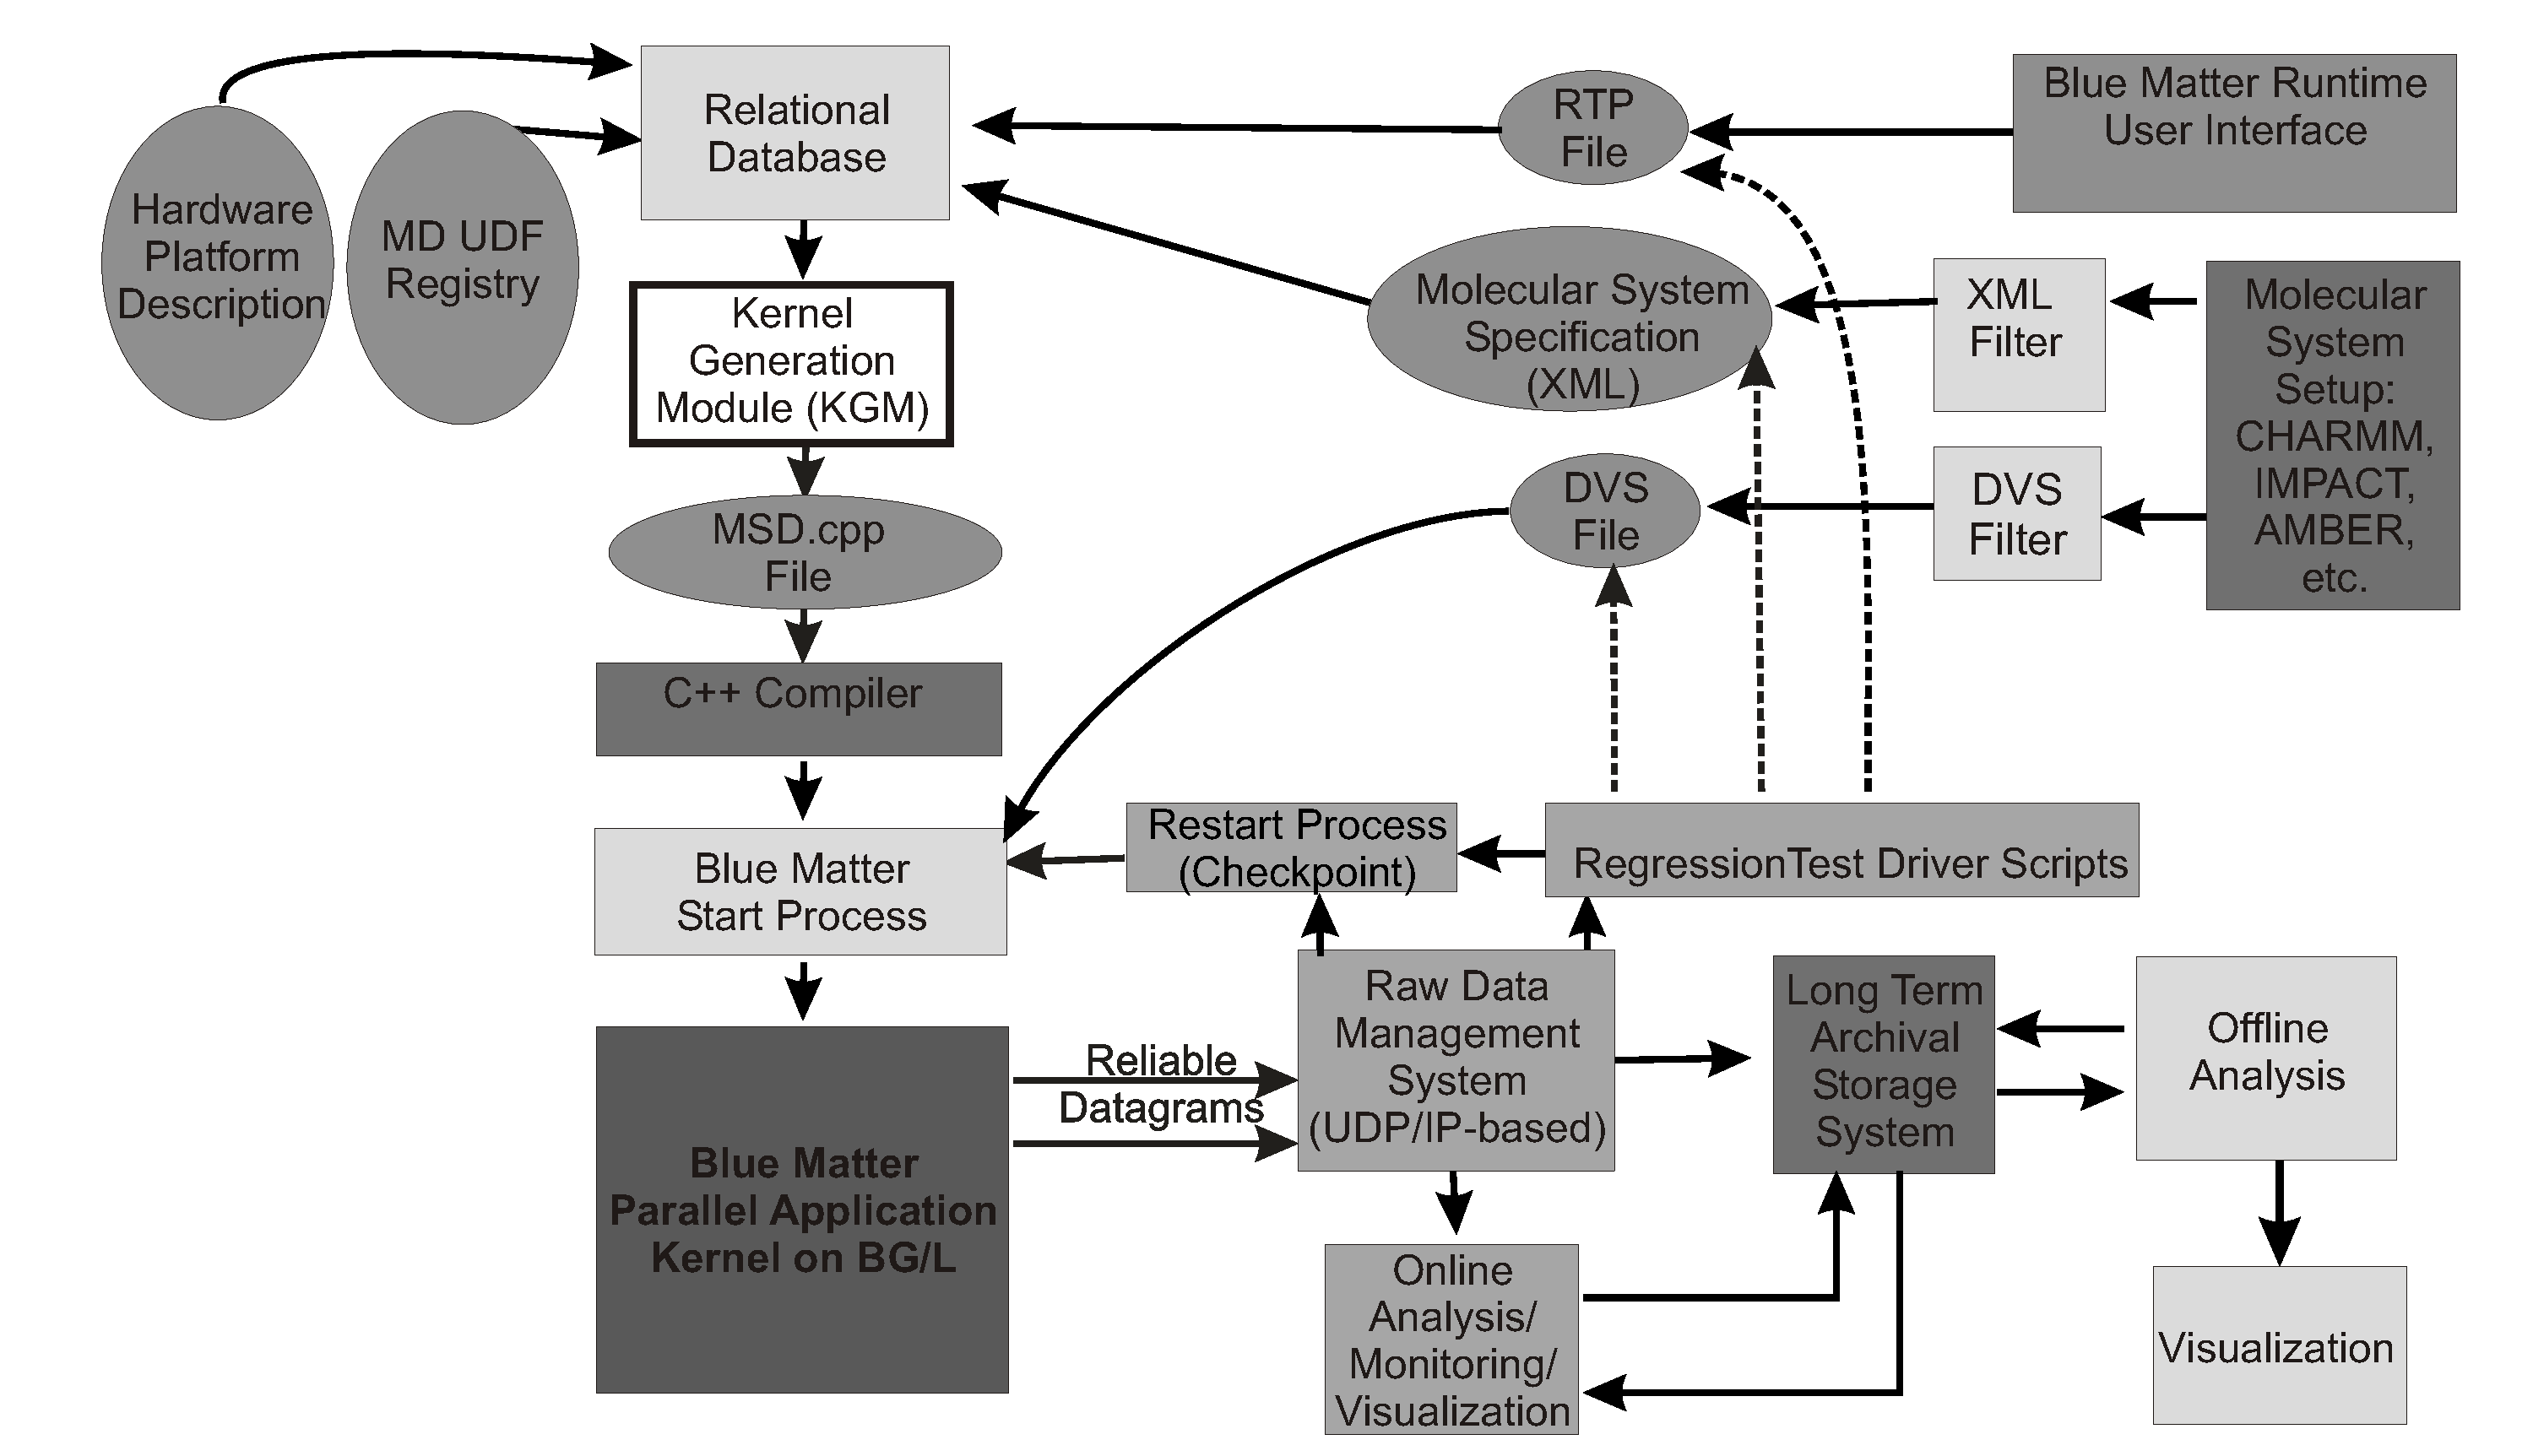
\includegraphics[keepaspectratio,
width=\textwidth]{BlueMatterFlow2_paper}
\caption{Overview of components and high level data flow within the application.}
\label{fig:bluematter_overview}
\end{sidewaysfigure}

\subsection{Set-up}

The set-up phase of Blue Matter collects all the non-dynamic
information required for a given simulation into a database and
generates the source code specific to that run.  First, the user runs
a commercially available simulation package
(e.g. CHARMm\cite{charmm:1998}, Impact\cite{impact},
AMBER\cite{amber:2002}, GROMOS\cite{gromos:1996}) to assign force
field parameters for the molecular system.  A package-specific filter
then transforms the output into an XML file that represents the
molecular system specification in a package-neutral form which is then
loaded into a relational database.  Relational constraints within the
database schema maintain internal consistency of the molecular system
where possible.  The user then specifies simulation parameters that
are stored in the relational database.  This phase of set-up
associates identifiers with both the inserted molecular system and the
specific simulation parameters and allows us to maintain an audit
path for our scientific and application development explorations
including the ability to execute {\em ad hoc} queries to find
molecular systems and parameter sets that have already been created.

Next, the kernel generation module (KGM) generates specialized source
code for the simulation using information stored in the database.
Since the KGM must recognize a wide variety of system specification
parameters and create corresponding code, it must encapsulate the
molecular dynamics domain knowledge.  The KGM generates a customized
molecular system definition (MSD) file containing parameters and
C++ code containing only the desired code paths in the
parallel kernel.  Minimizing the lines of source code allows more
aggressive and efficient optimization by the compiler.  Although many
parameters are built into the executable, others are provided at
runtime through the dynamic variable set (DVS) file, such as positions
and velocities.

\subsection{Generic Molecular Dynamics Framework}

Blue Matter encapsulates all molecular dynamics functions that
transform data in User Defined Functions (UDFs). The term UDF comes
from the database community where it refers to an encapsulated data
transformation added to the built-in functions that may be used during
a database query. Typically, these modules encapsulate domain specific
knowledge at the most fine grained level possible.  An example is the
standard coulomb UDF, which operates on two charge sites and yields
the force between them.

The UDF interface abstracts the calling context, allowing the
framework flexibility in organizing access to parameters and dynamic
variables.  For example, this flexibility allows the UDF driver
implementation to {\em tile} the invocations, an established technique
for improving data locality\cite{rivera:2000}.  In addition, the
interface enables the UDF function to be aggressively inlined into the
calling context.

%\subsubsection{UDF Adapters and Helpers}

UDF adapters and helpers are modules containing code that will be used
by more than one UDF.  An {\em adapter} is a module that implements
the framework UDF interface and also wraps another UDF.  A {\em
helper} is a subroutine that is called by a UDF via standard C++
method invocation interfaces and is passed values from the immediate
UDF context.  Adapters allow generic code to be encapsulated.  For
example, the generation of a virial for pressure control can be added
to a standard UDF by means of an adapter.  Adapters are written as C++
template classes taking an existing UDF as a parameter.

%\subsubsection{UDF Drivers}

UDFs represent pure data transformations that may be invoked from
several drivers.  The semantics of data movement are implemented in
the selection of UDF drivers.  For example, drivers exist to perform
pairwise $N^2$ operations (NSQ) as well as to run lists of operands.
Drivers used for a given simulation are selected during kernel
generation along with the appropriate UDFs that appear as template
parameters in the driver class.  Different drivers may be written for
different hardware platforms and/or load balancing strategies.

UDF drivers may be implemented in several ways while preserving the
same semantics.  For example, a set of drivers may support different
NSQ parallel decompositions.  The drivers themselves may be inherently
parallel with an instance on every node, each executing only a
fraction of the total number of UDF invocations. The implementation of
the UDF driver is where specific knowledge of the target architecture
is used to improve performance.  In the case of the Cyclops
architecture\cite{allen:2001}, which was the initial target hardware
platform for the Blue Gene project, the drivers had to be implemented
to issue enough independent work items to load 256 physical threads
per chip.  In the case of the BG/L architecture\cite{bgl_sc:2002}, it
is important to feed the processor instruction pipeline and to enable
reuse of framework recognizable intermediate values such as the
distance between two atoms.  Although these two hardware architectures
are quite different in their requirements, the design of Blue Matter
made it possible to adapt to both environments.

%\subsubsection{Parallel Programming Environment}

To facilitate early adoption of the experimental platforms which it
targets, the Blue Matter framework has been designed to have minimal
dependency on system software. The modularity of the framework allows
much of the program to run on a stable server.  To run the parallel
core in a new node environment requires a C++ compiler, a minimal C++
runtime, the ability to send and receive datagrams to external
machines, and a high performance communications mechanism.

Blue Matter can target two primary communications interfaces for
inter-node messaging: MPI and active messaging.  An explicit layer is
most appropriate when the application is operating in distinct phases
with relatively large grained parallelism.  For large node counts,
where scalability is bounded by the overhead of a very fine grained
decomposition, we target a simple active message interface. For
currently available machine configurations, the selection of
communications library is handled at an interface layer by selecting
either MPI or active message based collectives.  For BG/L, we are
integrating the framework drivers more directly with active messaging
to enable lower overhead and the overlapping of communication and
computation phases.

\subsubsection{Online Monitoring/Analysis}

The traditional view of a computational simulation has scientific code
running on a computer, periodically dumping results to a file system
for later analysis.  Blue Matter breaks from this standard model by
avoiding direct file i/o and instead communicating all results via
packets over a reliable datagram connection to analysis tools
listening on remote computers.  The resulting packet stream is the raw
datagram output (RDG).  Outputting a packet stream offloads a great
deal of the complexity of managing state and file formats from the
kernel to analysis tools that are less performance-critical. The
parallel kernel may emit packets out of sequence, and it is up is up
to the host monitoring module to marshal a consistent set of packets
for each time step, indicating the code is operating correctly and
allowing well-defined parsing.  Since the RDG stream is binary we
retain the full precision of the results for comparison and analysis.

Analyzing the RDG stream involves a combination of online processing
of the arriving packets and selective storing of pre-processed data
for efficient offline analysis.  For molecular simulations, the basic
online analysis involves parsing the packet stream and determining the
value of the energy terms at each time step, while storing the full
set of atom positions and velocities at regular intervals.  For each
time step containing atom positions we calculate, as a pre-processing
task, such features as the presence of hydrogen bonds, the secondary
structure, radii of gyration, and more.  The decision to calculate a
term online and store the result during the run depends on the expense
of the calculation and the size of the stored result.

The data stored during a computer simulation serve two distinct
purposes:
\begin{enumerate}
\item If the time evolution of the simulation is important, one
must record periodic snapshots of the simulation for later analysis
since the final state of the simulation does not convey the dynamic
path, or "trajectory," taken from the initial state.  These snapshots
need not include the full state of the system for later restart from
that point, but should contain all the information needed for
anticipated trajectory analysis.  In molecular simulations, saving the
trajectory is essential if the dynamic evolution of the system is
central to the experiment.
\item Apart from the scientific needs of
recording the system evolution there is also a practical need to store
the full system state for an exact restart of the simulation in case
of hardware or software error that either terminates the simulation or
causes inaccuracy in the output results.  In general, the state needed
for restart may be much larger than the state relevant to analysis
but, fortunately, molecular dynamics has relatively small state even
for large systems, dominated by the positions and velocities of all
the atoms (on the order of megabytes).
\end{enumerate}

\subsubsection{Post-Analysis and Data Management}

Since Blue Matter relies on a database for the set up of each system
to be run, the database can serve not only to define the simulation,
but to track the simulation runs of many scientists because the stream
contains a run identifier that directly binds to its full set of input
data in the database including: 1) the molecular system itself, 2) its
compile-time parameters, and 3) its initial configuration, i.e. atomic
positions and velocities, plus other state variables.  With all the
run information automatically tracked in the database without the need
for human input, powerful SQL queries across many independent runs
become possible.  The result is a high-integrity single source of
information in a database that serves as an experimental record to
track all the simulations, their parameters, and their results.

\subsubsection{Regression/Validation Infrastructure and Strategy}

A molecular dynamics simulation should be as fast as possible without
compromising the validity of the scientific results, and an important
part of MD code development is a suite of tools and test cases that provide
this validation\cite{gunsteren:1998}.  Blue Matter relies on a combination
of external regression tests that compare with other packages, internal
regression tests that track code changes, and validation tests that confirm
the scientific correctness of specific runs.  To facilitate the specification
and execution of these tests on a cluster of workstations we use
an environment that allows a concise specification of a
set of related runs, which makes it easier to create, modify, and run tests
that vary many parameters, despite the need to compile and build each
executable corresponding to each run. A more detailed description of these
tests follows.

Since Blue Matter supports a variety of standard force fields and
accepts input of molecular systems created by other MD packages, it is
essential to confirm that Blue Matter duplicates the energy components
and forces of those packages to a high degree of precision.  Blue
Matter uses the molecular systems and their corresponding energy
components and force results of an extensive suite of blocked amino
acids and peptides prepared with CHARMm, AMBER and Impact
(OPLS).\cite{brookssuite:2001} We use the set up phase of each MD
package to create a system in the corresponding force field, then use
Blue Matter to compute the energy terms and confirm the results agree
with the external regression suite.

One of the main validation checks on the code is to verify the extent
to which total energy is conserved. Although the total energy is not
strictly constant in time, the width of the total energy distribution
should vary quadratically with the time step size for dynamical
integrators based on simple Verlet-type algorithms and the total
energy should not display systematic drifts over time.  This is a
sensitive test of the correctness in the implementation of the
dynamics.  The procedure involves running the same molecular system
for the same amount of simulation time, using a range of time step
sizes, and calculating the root mean square deviation (RMSD) of the
total energy for each run.  A correct implementation will show RMSD's
that vary quadratically with time step to a fraction of a percent.
Since accumulated errors cause trajectories with different time steps
to depart from one another in phase space, we use short runs of a
fraction of a picosecond.  Other validation tests include checking the
density of water in a long constant pressure run with different water
models, confirming the equipartition theorem applies when constraints
such as rigid bonds are in use, confirming heat capacity estimates are
consistent those implied by the slope of energy-temperature curves
from temperature-controlled simulations, and simpler checks of
momentum and energy conservation in long runs.

The internal regression tests provide immediate feedback on code development,
but since Blue Matter outputs results in a lossless binary form, differences
can appear due to innocuous code changes such as a reordering of terms in a
summation.  In order to be sensitive to the larger changes in results that
indicate a bug, while insensitive to benign changes, a per-system tolerance
is incorporated into the tests that scales with system size and the length
of the regression test.  This helps automate the testing process since only
errors above threshold raise a flag that warrants inspection of the code.

\section{Issues in Mapping the Application onto the Machine}

\subsection{Interconnect Topologies (Torus and Tree)}

The replication unit for BG/L is a single ``system-on-a-chip''
application-specific integrated circuit (ASIC) to which additional
commodity DRAM chips are added to give 256 MB of external memory per
node.  512 of these replication units or ``cells'' will be be
assembled into an $8\times 8\times 8$ cubic lattice ``building block''
as shown in Figure~\ref{fig:brick}. The surfaces of this ``building
block'' (in effect, 6 sets of $8\times 8$ wires) connect to simpler
``link chips'' that send and receive signals over the relatively long
distance to the next ``building block''. A supervisory computer can
set up the links to partition the set of ``building blocks'' into the
sizes of lattice requested by the applications.  The result is three
dimensional torus wiring and the ability to route around blocks that
are out of service for maintenance. The ASICs also have connections
for a ``tree'' network. Each ASIC has a simple arithmetic-logic unit
(ALU) for the tree, enabling the tree to support ``add reduction''
(where each ASIC provides a vector of numbers; the vectors being added
element-wise to their partners at each node until a single vector
reaches the root; the vector is then broadcast back to all the
ASICs). ``max'', ``or'', ``and'', and ``broadcast'' are also supported
by the tree ALU.

\begin{figure}
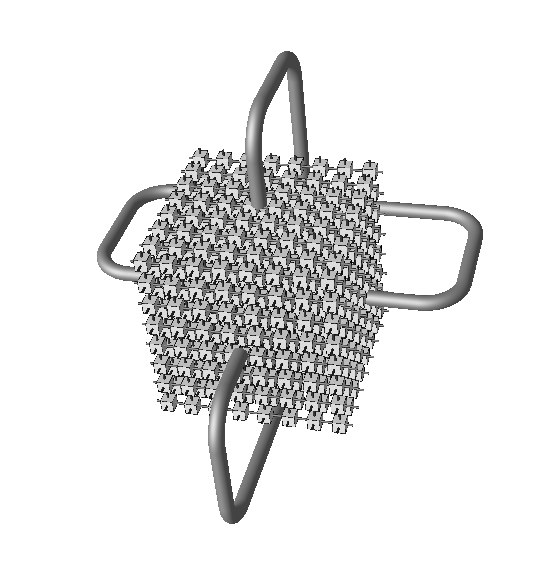
\includegraphics[keepaspectratio, width=\textwidth]{torus_dx}
\caption{View of a BG/L ``brick'' containing 512 nodes, showing the 3D
torus network}
\label{fig:brick}
\end{figure}

For the internal (torus and tree) networks, there is hardware
link-level error checking and recovery; an application on the compute
fabric is assured that a message sent from a node will arrive intact
and exactly once at its destination.  All links carry data in both
directions at the same time. The torus links carry 2 bits per CPU
clock cycle while the tree links carry 4 bits per CPU clock cycle.
For both networks, data are forwarded as soon as possible, with a
per-node latency equivalent to the time required to send a few bytes,
unless congestion on the outgoing link (torus and tree) or a wait for
partner data (tree reduction operations) forces data to be buffered.
There is no need for software intervention in any point-to-point
transmission.

\subsection{Efficient use of the Floating Point unit}
The Blue Gene/L CPU belongs to the IBM PowerPC family, and we use the IBM
VisualAge compiler with a modified ``back end'' to generate code for it.
Interaction with compiler developers has enabled better floating-point
optimization for the current POWER3 architecture as well as for Blue Gene/L,
which has resulted in a 30\% improvement in the performance of Blue Matter
when built to run on POWER3 machines.

On each ASIC there are 2 microprocessors. Each microprocessor is a
PowerPC 440 microcontroller to which two copies of a PowerPC-type
floating-point unit have been added. The CPU can run the normal
PowerPC floating-point instruction set and supports additional
instructions that operate on data in both floating-point units
concurrently. Each floating-point unit has its own set of 32 registers
at 64 bits wide.  All floating-point instructions (except ``divide'')
pass through a 5-cycle pipeline; provided there are no data
dependencies, one floating-point instruction can be dispatched per
clock cycle.  The PPC440 can dispatch 2 instructions per clock cycle,
thus peak floating-point performance would need 10 independent streams
of data to work on, and the program logic would require a
``multiply-add'' operation at every stage. This would account for a
``parallel multiply-add'' instruction dispatched every clock cycle; the
other dispatch slot in the clock cycle would be used for a load,
store, integer, or branch op in support of the program logic to keep
the floating-point pipeline busy and productive.  It is
straightforward to achieve this for a polynomial function $f(x)$ that
needs evaluation for 10 values of $x$, but for less regular code
kernels, or poorly controlled vector lengths, the fraction of peak
achieved depends on the skill of the programmer.  The unoptimized case
would dispatch only 1 instruction per clock cycle, not achieving any
parallelization to use the second floating-point unit, and not
exploiting the fused 'multiply' and 'add'; this would run at 5\% of
peak.  We have already implemented some computational kernels, such as
vector reciprocal square root, exponential, and inverse trigonometric
functions, that have been set up to exploit the double floating point
unit by avoidance of conditional branches and other strategies.

\subsection{Memory Hierarchy}

Each CPU has a 32 KByte instruction cache and a 32 kByte data
cache. The L1 line size is 32 bytes. There is no hardware support for
keeping the L1 caches coherent between the CPUs.  Associated with each
CPU is a prefetcher, known as L2, that fetches 128 bytes at a time
from L3. The ASIC contains 4 MBytes of DRAM as an L3 cache shared by
both CPUs.  The L1 can read 3 cache lines from L2 every 16 CPU clock
cycles, and concurrently write 1 cache line every 2 CPU clock
cycles. The L3 can keep up with this bandwidth from both CPUs.

The lack of coherency between the L1 data caches defines the ways in
which both CPUs can be used together. Those we foresee are
\begin{itemize}
\item Structured application coding, for example using
single-writer-single-reader queues and explicit memory synchronization
points to move data between CPUs in a well-defined way even though L1
is not made coherent by hardware.
\item CPUs used independently, as if they were on separate nodes
joined by a network.
\item Second CPU used as a Direct Memory Access (DMA)
controller. The first CPU would perform all the computation, flush
results as far as L3 cache, and set up DMA orders; the second CPU
would copy data between memory and the network FIFO interfaces. A
version of this mode would allow the second CPU to process active
messages, where an incoming torus packet contains a function pointer
and data, and the reception routine calls the function with the given
data. Parallel loads/stores to registers in the double floating point
unit request 16 bytes to be moved between registers and the relevant
level in the memory hierarchy every clock cycle.
\item Compiler-driven loop partitioning. A compiler would spot a
computationally-intensive loop (for example, 'evaluate the sine of
each element of a vector'); assign part of the vector to each CPU;
ensure that the relevant source data was flushed as far as L3; post
the second processor to start work, then start work on its own
portion; and synchronize with the second processor at completion.
\end{itemize}

\subsection{Identifying Concurrency in the Application\label{sect:concurrency}}

As a starting point for any discussion about how to map an application
onto a particular parallel architecture, it is essential to understand
the fundamental limits to concurrency present in the algorithm. Of
course, such estimates depend on the granularity of computation that
one is willing to distribute. One way to view the application
execution is as the materialization of a series of data structures
that are transformed from one into the other by computation and/or
communication. During a phase of computation, the number of possible
data-independent operations determine the concurrency present during
that phase of the application.  A view of this sort representing the
non-bonded force calculations in a molecular dynamics application
using the Ewald technique is shown in Figure~\ref{fig:ewald_data}.

Molecular Dynamics proceeds as a sequence of simulation time steps. At
each time step, forces on the atoms are computed; and then the
equations of motion are integrated to update the velocities and
positions of the atoms.  At the start, corresponding to the leftmost
box in Figure~\ref{fig:ewald_data}, the positions and velocities of
all the particles are known and a data structure indexed by the
particle identifier $l$ can be distributed using any ``hashing''
function of $l$ with the maximum possible number of hash slots equal
to the number of particles, $N$.  Both atom and volume based
decompositions are possible.

\begin{sidewaysfigure}[p]
\begin{center}
\includegraphics[keepaspectratio, width=\textwidth]{p3me0}
\caption{Data dependencies of the major components of a molecular
dynamics application using the Ewald Method}
\label{fig:ewald_data}
\end{center}
\end{sidewaysfigure}

Following the upper branch of data dependencies, the next phase
involves computation of all the pairwise forces between particles.
This requires a data structure to be materialized that contains all
pairs of particle positions so that the computation of the pair forces
can take place.  This structure can be indexed by a pair of particle
identifiers $l$ and $m$ and indicates that distribution over a much
larger number of hash slots, $N^2$, is possible although the finite
range cut-offs used for the pair potentials means that the actual
number of non-vanishing pair computations is much smaller than $N^2$.
This is the phase of the application where an ``interaction''
decomposition is often used\cite{plimpton:1995}.  Next, a reduction is
required to sum up the pairwise forces on each particle so that a data
structure containing the total force on each particle, indexed by the
particle identifier $l$ can be created.

Along the lower branch of data dependencies, the calculation of the
Ewald sum requires exponentials that are functions of particle
position and $\mathbf{k}$-vector value.  The $\mathbf{k}$-vector
values are fixed and the number required is determined by the accuracy
required in the Ewald sum.  The data structure containing these values
is indexed by the particle identifier $l$ and the $\mathbf{k}$-vector
index $\alpha$.  Next, components of the Fourier transform of the
charge density need to be computed, which requires a reduction of the
exponentials according to the $\mathbf{k}$-vector index $\alpha$.  The
data structure containing the reciprocal space contributions to the
force (indexed by particle identifier $l$ and $\mathbf{k}$-vector
index $\alpha$) requires both the Fourier transform of the charge
density and the exponentials computed earlier. These contributions
must also be added into the total force on each particle. Finally, the
data structure containing the total force on each particle, indexed by
$l$, can be used to propagate the dynamics
and give new values for the position and velocity of each particle.

The number of independent data items at each stage in this process is
as follows:
\begin{itemize}
\item For stages that are partitionable by particle identifier,
the number of independent data items is $N$, the number of particles.
\item For the pair force computation stage, which is partitionable by
pairs of particle identifiers, the theoretical limit on the number of
data items is $N^2$, but because of the finite range of the force
expressions typically used in these computations, the actual number of
independent computations possible is $\approx
(1/2)\,N\,\rho\,(4/3)\,\pi\,r_c^3$ where $\rho$ is the number density
of atoms and $r_c$ is the cutoff radius, beyond which the force between
two particles vanishes.
\item For the computations of the exponentials and the reciprocal
space force that are partitionable by particle identifier $l$
and $\mathbf{k}$-vector index $\alpha$, the number of independent data
items is the product of the number of $\mathbf{k}$-vectors required
(typically a few hundred) and $N$, the number of particles.
\item The computation of the Fourier transform of the charge density
is partitionable by the $\mathbf{k}$-vector index $\alpha$, again
giving a few hundred independent data items.
\end{itemize}

A similar analysis can be carried out for mesh-based Ewald techniques
such as P3ME in which the solution of Poisson's equation is
accelerated through use of the fast Fourier transform (FFT) after
approximating the actual charge distribution by weights on a regularly
spaced mesh.  In the variant of P3ME that we will consider here, the
{\em analytic} method, the meshed charge distribution is actually
convolved with four kernels to give the electrostatic potential as
well as the three components of the electric field within the
simulation volume.  This requires a single forward 3D-FFT followed by
independent multiplications by each of the four kernels and then four
inverse 3D-FFTs (one for each kernel).  The parallel 3D-FFT itself
involves significant communication that will be described below.

\section{Case Studies of Parallel Decompositions and Scalability Projections}

In this section we use relatively simple models to explore the
scalability of various decomposition/parallelization schemes for
molecular dynamics of macromolecular systems on BG/L.  In studies of
the scaling of fixed size problems to large numbers of nodes, there is
no expectation that ideal scaling will be observed.\cite{Taylor:1997}
However, for a specified problem size, useful parallel speed-ups
should be achievable on a range of node counts with the upper limit on
node count being determined by the portion of the computation with the
least favorable scaling properties (Amdahl's law).  Our intent is to
use these model calculations to assist in making decisions about the
relative viability of various approaches and to assess the balance
between computation and communication within these approaches, {\em}
not to make absolute performance predictions.

In the examples that follow, our focus is on communications patterns
that map closely to the hardware capabilities of the BG/L architecture
because we want to keep the potential for software overheads to a
minimum.  Some of the communications estimates used below are derived
from work on a network simulator developed by members of the BG/L team
while others, such as the capabilities of the tree network are taken
directly from the designed capabilities of the
hardware.\cite{bgl_sc:2002} Cycle count estimates for computational
kernels are taken from the output of the IBM C++ compiler that targets
the BG/L architecture or from estimates of the time required for
memory accesses.  The assumptions built into the examples that follow
are:
\begin{itemize}
\item System software overheads are neglected
\item No overlap between computation and communication is utilized
\item Only one CPU per node is available for computation
\item Memory access times are neglected except where we have been able
  to identify them as dominating the time for computation (only for
  integration of the equations of motion).
\end{itemize}

Since all of our work requires accounting correctly for the effects of
the long range interactions in the system, the first case study
concerns the properties of a three-dimensional FFT on the BG/L
architecture. The two other case studies, which deal with different
mappings of molecular dynamics onto the BG/L hardware, both assume
the same set of FFT-based operations to support the P3ME method.
Also, the projections made in these case studies neglect the
contributions of bonded force calculations to the total computational
burden since they represent relatively small fractions of the total
and can be distributed well enough to keep their contribution to the
per node computational burden small.  The parameters used in the
models are defined in Table~\ref{tab:model_params}.  Although the
actual machine has hardware support for partitioning down to a
granularity of 512 nodes, we include smaller node counts in our model
for illustrative purposes. Occasional ``anomalies'' visible in in
graphs of the performance are due to the fact that since the machine
is partitionable into multiples of eight nodes in each dimension, many
node counts will be comprised of non-cubical partitions which affect
the performance of the torus communications network.

\begin{table}
\begin{tabular}{|l|l|}\hline
Parameter & Description\\ \hline\hline
\verlettime & Execution time for dynamics propagation of a single site
\\ \hline
\sitecount & Total number of sites \\ \hline
\rcutoff & Cut-off distance for non-bond forces \\ \hline
\density & Number density of system \\ \hline
\nodecount & Node count \\ \hline
\allreducetime & Execution time for {\tt AllReduce} of forces \\ \hline
\globalizepostime & Execution time for position globalization \\ \hline
\meshsize{i} & Dimension of charge mesh in dimension $i$. $\meshsize{i} = L_i/h$ \\ \hline
\nonbondtime & Execution time for pairwise non-bonded interactions \\ \hline
\pmetime & Execution time for P$^3$ME including FFT \\ \hline
\end{tabular}
\caption{Model Parameters}
\label{tab:model_params}
\end{table}

\begin{table}
\begin{tabular}{|l|l|l|l|l|}\hline
System Size (atoms)& 5000& 10,000& 20,000& 30,000 \\ \hline
Cycle Count& $3.097\times 10^9$& $3.454\times 10^9$& $4.168\times 10^9$& $4.881\times 10^9$\\ \hline
Time (sec.)& 4.42& 4.93& 5.95& 6.97\\ \hline
\end{tabular}
\caption{Single node cycle counts/time step and projected time/time
  step (at 700MHz nominal clock speed) for global force reduction
  method.}
\label{tab:gfr_uniproc}
\end{table}

In the model used to produce
Figures~\ref{fig:estimate_speedup} and
\ref{fig:estimate_contributions}, the contributions to \pmetime\
comprise one forward and four inverse 3D real-valued FFTs to give the
electrostatic potential and the three components of the electric field
using the analytic method as described in
Section~\ref{sect:concurrency}.

\subsection{Three Dimensional Fast Fourier Transform}

The communication estimate for the 3D FFT assumes that three
all-to-all communications within a processor plane or row are required
for each FFT or its inverse.  From simulations of the BG/L torus
network, the following estimate for the time (in processor cycles)
required for all-to-all communication of data that is distributed over
a set of nodes in a line, plane, or volume is
obtained\cite{bgl_comm:2002}:
\begin{displaymath}
T_{all-to-all} = \frac{V_{received}\,\overline{N}_{hops}}{N_{links}\,BW\,f}
\end{displaymath}
where $V_{received}$ is the volume of data received by each node,
$\overline{N}_{hops}$ is the average number of hops required (for a
three dimensional torus where each dimension is $p$,
$\overline{N}_{hops} = p/4$ for all-to-all in a line,
$\overline{N}_{hops} = p/2$ for all-to-all in a plane, and
$\overline{N}_{hops} = 3p/4$ for all-to-all in a volume), $N_{links}$ is
the number of links available to each node ($2$ for linear
communication, $4$ for planar communication, and $6$ for volumetric
communication), $BW$ is the raw bandwidth of the torus per link (2
bits per processor clock cycle), and $f$ is the link utilization
(assumed to be 80\%).  Note that the time required for all-to-all
communication is independent of the dimensionality of the
communication because of the compensating effects of the average hop
count and the number of links available for the communication.

For the target scientific application, system sizes are such that a
mesh size of $128\times 128\times 128$ is most common.  For small node
count systems, a ``slab'' decomposition of the FFT onto an array of
processors is most efficient.  However, this would only allow mapping
of the FFT onto partitions with at most 128 nodes.  In principle,
there is plenty of work to distribute over a much larger number of
nodes since if we assume that the 1D FFT is not to be parallelized,
each stage in the 3D FFT requires $\meshsize{mesh}^2$ 1D FFT
computations.  This does require significantly more communication than
a ``slab'' decomposition.

Since BG/L is a torus/mesh machine, it is natural to use a volume
decomposition to map the 3D mesh domain onto the machine.  Assuming
that the domain mesh dimensions are $\meshsize{0}\times
\meshsize{1}\times\meshsize{2}$ and that the machine partition size is
$p=p_0\times p_1\times p_2$ then each node will have responsibility
for $(\meshsize{0}/\nodemeshsize{0})\times
(\meshsize{1}/\nodemeshsize{1})\times (\meshsize{2}/\nodemeshsize{2})$
mesh points.  Estimates of the various contributions to a $128\times
128\times 128$ 3D-FFT are shown in Figure~\ref{fig:estimate_fft} as a
function of node count.  For this choice of mesh size, there are
$128\times 128=16,384$ one-dimensional FFTs to be distributed over the
nodes, which makes scaling the FFT beyond $16,384$ nodes impossible
without distributing the individual one-dimensional FFTs as well.
Note that the computation dominates communication until the node count
exceeds 512 and the FFT continues to speed up until hardware latencies
begin to dominate for node counts in excess of $4096$.  These
latencies become important because the amount of data sent from each
node as part of the all-to-all communication drops as the node count
increases.


\begin{sidewaysfigure}[p]
\begin{center}
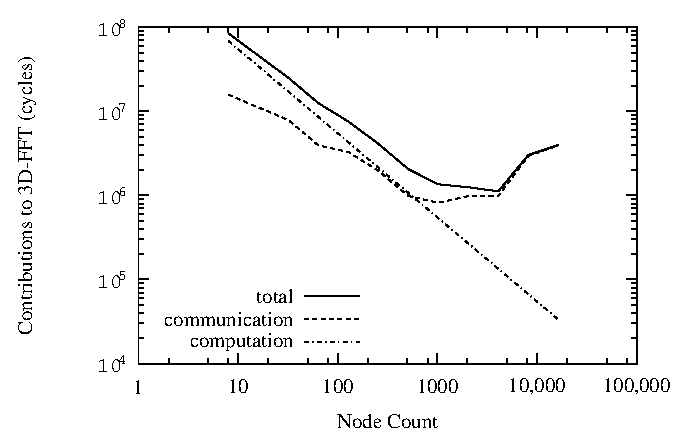
\includegraphics[keepaspectratio, width=\textwidth]{estimate_fft}
\caption{Computation and communications estimates for a 3-dimensional
FFT on a $128\times 128\times 128$ mesh.  These estimates assume use
of the BG/L torus network to carry out the required communication.
Note that for this mesh size, the FFT cannot scale beyond 16,384 nodes
because at each phase in the 3D-FFT calculation, there are $128\times
128$ individual one-dimensional FFTs to be distributed over the nodes.
Also, communication dominates computation for node counts above 512
and hardware latencies actually decrease performance with increasing
node count above about 4000 nodes.}
\label{fig:estimate_fft}
\end{center}
\end{sidewaysfigure}

\subsubsection{Global Force Reduction (GFR)\label{sect:gfr}}

One simple parallel decomposition for real space molecular dynamics
focuses on global force reduction. This allows the pairwise
interactions to be arbitrarily partitioned amongst nodes to achieve
load balance.  Once per time step, all nodes participate in a
summation all-reduction implemented over the global tree network
(equivalent to standard global reduce followed by a broadcast) with
each node contributing the results of its assigned interactions.
Given access to net force on each particle and the current positions
and velocities of each particle, each node can replicate the numerical
integration of the equations of motion for each particle to give every
node a copy of the updated full configuration of the system.  Since
each node has access to the full configuration of the system, this
decomposition can work with versions of the P3ME method that use only
a subset of the nodes for the FFT computation.

GFR has the following advantages:
\begin{itemize}
\item Load balancing of the non-bonded force calculation is
  straightforward.
\item Double computation of the non-bonded forces can be avoided.
\item P3ME can be supported in a number of decompositions including
  using only a subset of nodes for the P3ME portion of the computation
  since the computed forces are made visible on all nodes.
\end{itemize}
Drawbacks to GFR are:
\begin{itemize}
\item The replication of the dynamics propagation on all nodes
  represents non-parallelizable computation.
\item The force reduction itself is non-scalable as implemented on the
  global tree.
\item The implementation of a floating point reduction on the global
  tree network requires additional software overhead.  In our model,
  two reductions are required--the first establishes a scale through a
  16 bit/element comparison reduction while the second carries out a
  summation reduction with scaled fixed point values (64 bits/element).
\end{itemize}

It is possible to reduce the replication of dynamics propagation by
using some form of volume decomposition and Verlet lists.  Using these
facilities, each node need only propagate dynamics for atoms either
homed on that node or within a cutoff distance (or within the guard
zone when using Verlet lists).

\subsubsection{Global Position Broadcast Decomposition\label{sect:gp}}

Another possible decomposition that leverages the capabilities of the
global tree network on BG/L is based on a global position broadcast
(GPB). Local force reductions will be required, but their near
neighbor communications burden will be neglected in this model.  A
functional overview of the GPB class of decompositions is as follows.
Once per time step the atom position vector will be bit-OR all-reduced
(OR reduce, then broadcast) via the global tree network.  However, for
P3ME this method will also require near neighbor force reduction since
atoms will generate forces from FFT mesh points on nodes other than
their home node.  Because of this, it is advantageous to maintain a 3D
spatial mapping of atoms/fragment to nodes in BG/L.  An issue with
using near neighbor point-to-point messages to bring in the forces
from the P3ME/FFT mesh points off node will be figuring out when all
the forces have been received.  To handle this, for each fragment
homed on a node, a deterministic algorithm must yield an expectation
of the exact number of forces to wait for.  In this method, we
partition both the force generating operations as well as the
integration parts of the loop - each node only propagates dynamics for
those sites/fragments that are locally homed.

In this initial version of the model for global position broadcast,
double computing of forces will be assumed as well as ideal load
balancing of real-space non-bonded forces.  The model corresponding to
these assumptions is
\begin{eqnarray}
T_{non-bond} & = & \frac{1}{\nodecount}\,\sitecount\,\verlettime \nonumber \\
       &   & \mbox{} +
       \big(\frac{\sitecount}{\nodecount}\big)\,\frac{4}{3}\,\pi\,\rcutoff^3\,\density\,\nonbondtime
       \nonumber \\
       &   & \mbox{} + \pmetime \nonumber \\
       &   & \mbox{} + \globalizepostime \nonumber
\end{eqnarray}.

The speedups as a function of node count are shown in
Figure~\ref{fig:estimate_speedup} for a set of system sizes while the
individual contributions to the total time required for the non-bond
interactions in a system of $30,000$ particles are shown in
Figure~\ref{fig:estimate_contributions}.

\begin{sidewaysfigure}[p]
\begin{center}
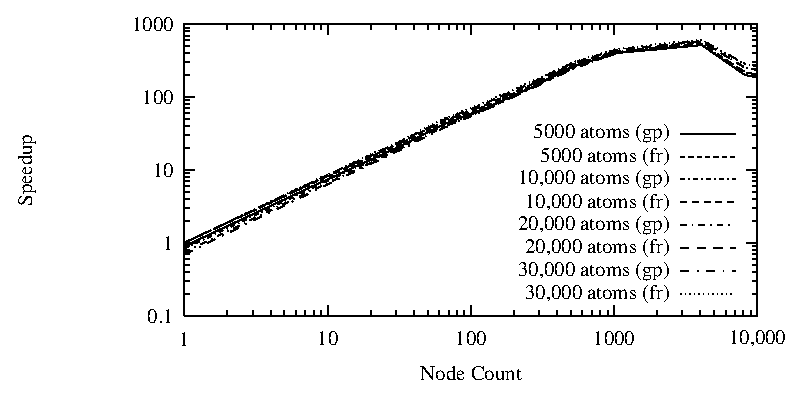
\includegraphics[keepaspectratio, width=\textwidth]{estimate_speedup}
\caption{Speedup estimates for molecular dynamics on BG/L using two
different parallelization schemes, position globalization (gp) and
global force reduction (gfr). All speedups are computed with reference
to the global force reduction implementation (for each system size) on
a single node given in Table~\ref{tab:gfr_uniproc} since this is the
fastest uniprocessor implementation. Note that the observed speedup is
only weakly dependent on system size.
These estimates assume ideal load balancing and do not include the
contributions for bonded interactions since the size of these
contributions are a very small fraction of the computational burden as
well susceptible to a reasonable degree of distribution.  The
molecular dynamics methodology assumed here is P3ME using a Verlet
integrator.}
\label{fig:estimate_speedup}
\end{center}
\end{sidewaysfigure}

\begin{figure}[p]
\begin{center}
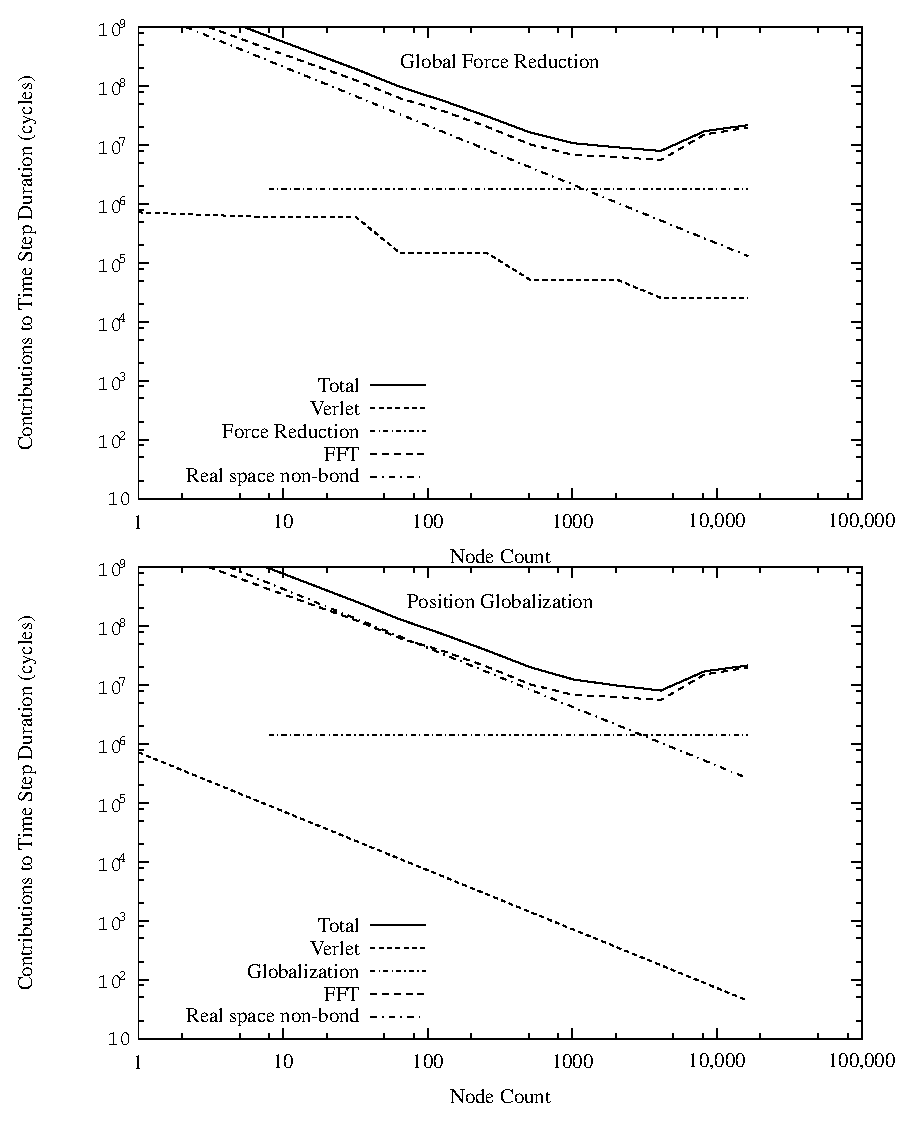
\includegraphics[keepaspectratio, height=7in]{estimate_contributions}
\caption{An estimate of the contributions of various computational and
communications operations to the total number of cycles required to
carry out a time step on a $30,000$ atom system is shown as a function
of node count for two different parallelization schemes, position
globalization (gp) and global force reduction (gfr). At very large
node counts, the performance of both schemes is limited by the
communications time required for the 3D FFT rather than the global
position broadcast or force reduction.}
\label{fig:estimate_contributions}
\end{center}
\end{figure}

\subsection{Discussion}

The data shown in Figure~\ref{fig:estimate_speedup} indicate that in
the range of system sizes of interest, both parallel decompositions
discussed above have projected speedups of $\approx 250$ at $512$
nodes for a parallel efficiency of $\approx 50$\%.  At sufficiently
large partition sizes the communications required by the 3D FFT
dominates the time step duration and eventually this communications
cost becomes dominated by hardware latency (leading to the loss of
parallel speedup seen in
Figures~\ref{fig:estimate_fft},~\ref{fig:estimate_speedup},
and~\ref{fig:estimate_contributions}) because of the decreasing amount
of data sent in each message.  Because of this the tree-based
globalization communication costs do not become an issue and the simple
parallelization schemes considered here appear to be viable for node
counts up to several thousand.

These projections were made from models constructed with the
assumptions that no overlap is possible between communication and
computation and that only one CPU on each node is available for
computation.  If we can implement these decompositions in ways that
allow us to bypass any of these assumptions, it should be possible to
increase the realized computational rate.

\section{Areas for Exploration}

\subsection{Multiple Time Step Integration}

Any methods that increase the ratio of simulation time to
computational effort through algorithmic means are extremely
attractive candidates for investigation.  The development of methods
to integrate the equations of motion in a way that takes account of
the multiple time scales present in a molecular dynamics simulation
provides a means of reducing the number of times that expensive long
range force evaluations need to take place during a fixed amount of
simulation time.\cite{tuckerman:92,zhou:2001} Implementing these
methods efficiently in the context of the parallel decompositions
discussed above may require some modifications to the implementation
of those decompositions, but the potential benefits in a parallel
program are large\cite{phillips:2002} especially when an appropriate
decomposition of the electrostatic forces is used in combination with
an efficient algorithm for periodic electrostatics like
P3ME.\cite{zhou:2001}

\subsection{Alternatives for periodic electrostatics.}

Several algorithms have been developed and extensively tested for
efficient evaluation of electrostatic forces, but improving already
existing and developing new algorithms remains an area of active
research. These algorithms differ in the degree of implementation
complexity, scalability with the number of particles, and suitability
for parallelization as defined by scaling with the number of nodes
used.

The particle-particle-particle-mesh (P3ME) method\cite{hockney:1988}
uses FFT methods to speed up calculation of the reciprocal space part.
The P3ME method has good scalability with system size since the computational
cost grows as $N\,\log N$, and this is currently the most popular approach 
used in MD packages. Unfortunately, parallelization of the
P3ME method is limited by the properties of the FFT algorithm, which
involves significant communications between nodes.

Many algorithms can be classified as 
tree methods or multiple grid methods. Both approaches are
similar in that they hierarchically separate interactions based on
their spatial separation. The tree methods separate particles into
clusters based on their relative distance, while the multi-grid methods use
grids of different coarseness to approximate the smooth part of the
potential between pairs of particles.

A well-known example of a tree method is the Fast Multipole
Method\cite{greengard:87}, in which distant particles are grouped in
clusters and the effect of distant clusters is approximated using
multipole expansion. The scaling of this algorithm is $O(N)$. A
typical implementation of this algorithm is usually rather expensive,
and therefore it becomes faster than the P3ME method only at
relatively large system sizes.

Another method developed by Lekner\cite{lekner:1991} provides an
alternative to Ewald summation and related techniques for handling
electrostatic interactions between particles in a periodic box. The
effect of all the periodic images is included in an effective
pair-wise potential. The form of this potential allows a product
decomposition to be applied\cite{sperb:1999}. The rate of convergence of
the resulting series depends strongly on the ratio of the separation
between particles in one of the dimensions and the periodic box
size. The hierarchy of scales in this method is achieved by adding and
subtracting images of charges to create periodic boundary conditions
in a box of half the spatial extent in one of the dimensions. Then the
procedure is repeated for several scales of box sizes.  The scaling of
this method with the particle number is $O(N\,\log N)$. Studies of the
efficiency of this method show promising results in comparison with
other methods in cases where the accuracy of the electrostatic
interaction calculations is relatively high\cite{strebel:2001}.


\section{Summary and Conclusions}

We have described the architecture of the Blue Matter framework for
biomolecular simulation being developed as part of IBM's Blue Gene
project as well as some of the features of the Blue Gene/L machine
architecture that are relevant to application developers,
particularly, issues and approaches associated with achieving
efficient utilization of the double floating point unit.  This work in
collaboration with the IBM Toronto compiler team has not only improved
code generation for BG/L, but has also led to significant
improvements, 30\% or more, in the performance of Blue Matter on the
existing Power3 platform.  In order to guide our development efforts
and algorithmic investigations, we have explored two parallel
decompositions that leverage the global tree interconnect on the BG/L
platform as well as a distributed implementation of a
three-dimensional FFT (required for the most widely used treatment of
periodic electrostatics in molecular simulation) using the BG/L torus
network through modeling.

Our estimates indicate that a 3D-FFT on a $128\times 128\times 128$
mesh remains computation dominated up to a partition size of 512 nodes
and that significant speed-ups are realizable out to larger node
counts.  The two decompositions described here, position globalization
and global force reduction, both rely on reductions implemented via
BG/L's global tree.  Both schemes have projected parallel efficiencies
of about 50\% out to 512 nodes for system sizes in the range of 5000
to 30,000 atoms and the time required to compute a single time step
becomes dominated by communications latency effects in the 3D-FFT
implementation for node counts above $\approx 4000$.  Given that the
simulation experiments under consideration require multiple
independent or loosely coupled molecular simulations, we conclude that
these results indicate that FFT-based particle mesh techniques are a
reasonable first approach to implementing a molecular simulation
application that targets BG/L.  As hardware becomes available, we will
be able to validate our estimates, assess the impact of system
software overheads, explore whether some overlap of communication and
computation is possible, and assess the possibility of using both CPUs
on a BG/L node for computation.

%\begin{thebibliography}{00}

% \bibitem{label}
% Text of bibliographic item

% notes:
% \bibitem{label} \note

% subbibitems:
% \begin{subbibitems}{label}
% \bibitem{label1}
% \bibitem{label2}
% If there is a note, it should come last:
% \bibitem{label3} \note
% \end{subbibitems}

%\bibitem{}

%\end{thebibliography}
\bibliography{../bibliography/md}

\end{document}


:
